% Beamer template
% Author: Ozgur Taylan TURAN
% Delft University of Technology

\documentclass[aspectratio=169]{beamer}
% PACKAGES
\usepackage[english]{babel}
\usepackage{graphicx}
\usepackage{animate}
%\usepackage{calc}
\usepackage{calligra}
\usepackage[absolute,overlay]{textpos}
\usepackage[T1]{fontenc}
%\usefonttheme{serif}
\usefonttheme{professionalfonts}
\usepackage{amsmath}
\usepackage{palatino}
\usepackage{mathpazo}
\usepackage{graphicx}
%\usepackage{subfig}
\usepackage{tikz}
\usetikzlibrary{shapes,arrows}
\usepackage{xcolor}
\usepackage[T1]{fontenc}
%\usefonttheme{serif}
%\usepackage{titling}
\usepackage{graphicx}
%\usepackage{subfig}
%\usepackage{tikz}
%\usetikzlibrary{shapes,arrows}
\usepackage{mathtools}
\usepackage{cancel}
% CUSTOM PACKAGES
\usepackage{/home/taylanot/texmf/tex/beamerthemetot}
\input{/home/taylanot/texmf/presentation/tune.tex}

 % COVER PAGE INFO   
\newcommand{\mytitle}{\color{White}\huge{\textbf{Lab Talk \#4}}}

\newcommand{\mysubtitle}{\color{Pink}\huge{\textbf{"Learning" Learning Curves}}}
\newcommand{\intro}{\color{Pink}\huge{\textbf{Introduction}}}
\newcommand{\pr}{\color{Pink}\huge{\textbf{Problem Definition}}}
\newcommand{\res}{\color{Pink}\huge{\textbf{Initial Questions}}}
\newcommand{\plans}{\color{Pink}\huge{\textbf{Plans}}}
\newcommand{\thnx}{\color{Pink}\huge{\textbf{Thanks!}}}

\newcommand{\myauthor}{\color{White}\textcalligra{\LARGE Ozgur Taylan Turan}}
\newcommand{\authorlabel}{\small O.T. Turan}

\author{\authorlabel}

\setlength\bibitemsep{0.3cm} % space between entries in the reference list
\renewcommand{\bibfont}{\normalfont\scriptsize}
\renewcommand{\cite}[1]{\footnote<.->[frame]{\fullcite{#1}}}
\setbeamertemplate{bibliography item}{}
\bibliography{/home/taylanot/Dropbox/archive_bib/SPKR.bib,/home/taylanot/Dropbox/archive_bib/LearningCurve.bib }

\newcommand{\ispace}{\mathbb{X}}
\newcommand{\ospace}{\mathbb{Y}}
\newcommand{\hypspace}{\mathbb{H}}
\newcommand{\hyp}{h}
\newcommand{\inp}{x}
\newcommand{\out}{y}
\newcommand{\algo}{\mathcal{A}}
\newcommand{\nsamp}{N}
\newcommand{\nsampi}{N_i}
\newcommand{\samp}{\mathcal{D}_\nsamp}
\newcommand{\sampi}{\mathcal{D}_{\nsamp_{i}}}
\newcommand{\prob}{\mathcal{P}}
\newcommand{\probspace}{\mathbb{P}}
\newcommand{\pred}{\hat{y}}
\newcommand{\loss}{\mathcal{L}}
\newcommand{\risk}{\mathcal{R}}
\newcommand{\avgrisk}{\bar{\risk}}
\newcommand{\expect}{\mathbb{E}}
\newcommand{\Zpos}{\mathbb{Z^+}}
\newcommand{\R}{\mathbb{R}}
\newcommand{\task}{\mathcal{T}}

\newcommand{\algolr}{\mathbb{M}}
\newcommand{\lc}{\mathcal{C}}
\newcommand{\nlim}{k}
\newcommand{\nsamplr}{Q}
\newcommand{\numlc}{M}
\newcommand{\samplr}{\mathcal{Z}}
\newcommand{\model}{\mathcal{M}}
\newcommand{\hilbert}{\mathbb{H}}
\newcommand{\data}{\boldsymbol{\alpha}}
\newcommand{\func}{\boldsymbol{\beta}}
\newcommand{\mR}{\mathbb{R}}

\begin{document}
% COVER PAGE
{
\def\beamer@entrycode{\vspace*{-\headheight}}
\setbeamertemplate{frametitle}[default][center]
\setbeamertemplate{navigation symbols}{}
\usebackgroundtemplate{
\includegraphics[width=\paperwidth,height=\paperheight]{cover/coverart.pdf}}

\begin{frame}[plain] 

\begin{minipage}{\textwidth}
	\centering{\mytitle} \\
	%\vspace{1cm}
	%\centering{\mysubtitle} \\
	\vspace{1cm}
	\centering{\color{White}November 15, 2021} \\
	\vspace{1cm}
	\centering{\myauthor}\\
\end{minipage}
\end{frame}
}


\begin{frame}
	\centering
	\mysubtitle
\end{frame}

\begin{frame}
	\centering
	\intro
\end{frame}

\section{Introduction}
\begin{frame}{Learning Curves}
  \begin{minipage}{0.5\textwidth}
    \begin{itemize}
      \item<1> Not \textit{Training Curves}
      \item<2> Generalization Performance for a given $N$ number of training points 
    \end{itemize}
  \end{minipage}%
  \begin{minipage}{0.5\textwidth}
    \centering
    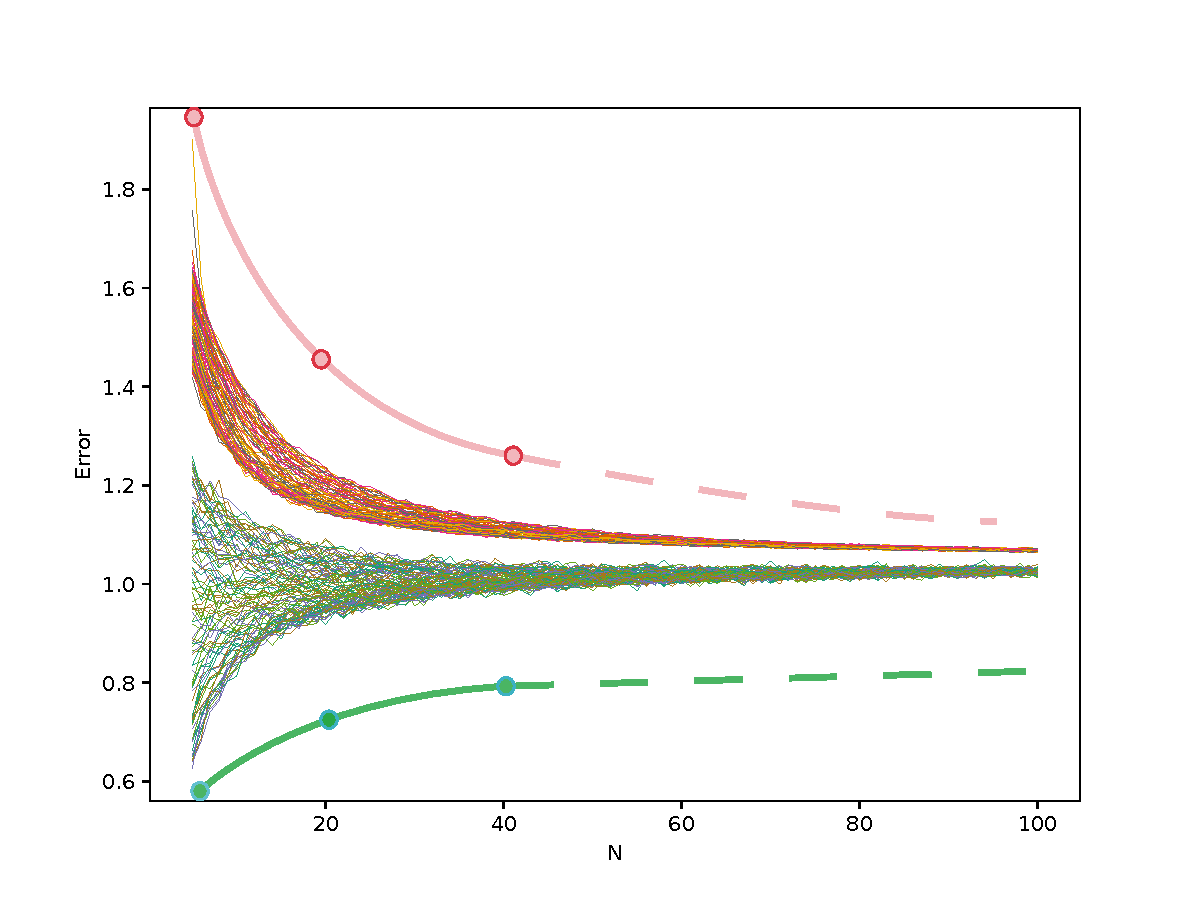
\includegraphics[width=\textwidth]{figures/lc.pdf}
  \end{minipage}
\end{frame}

\begin{frame}{Learning Curves "formally"}
\begin{minipage}{0.5\textwidth}
  \begin{itemize}
    \item $\avgrisk(\algo, \nsamp) = \underset{{\samp}}\expect\risk(\algo(\samp)))$
  \end{itemize}

  \vspace{0.5cm}

  $\samp:=(\inp,\out)_{i=1}^{N}$

  \vspace{0.5cm}

  $\algo(\samp)\to\hyp$

  \vspace{0.5cm}

  $\risk(\hyp) := \int\loss(\out,\pred)d\prob_{\samp}$ 


\end{minipage}%
  \begin{minipage}{0.5\textwidth}
  \centering
  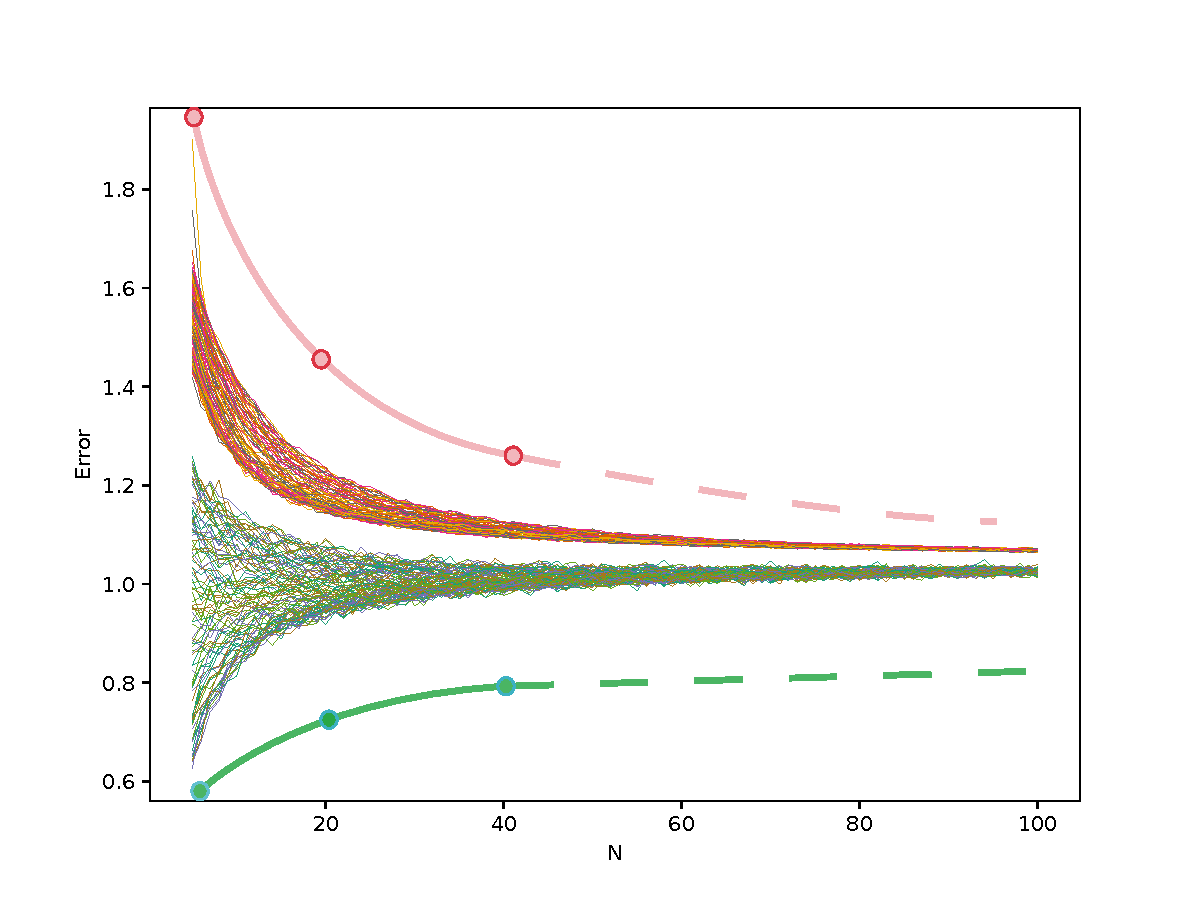
\includegraphics[width=\textwidth]{figures/lc.pdf}
\end{minipage}
\end{frame}

\begin{frame}{Learning Curves Importance}
  \begin{minipage}{0.5\textwidth}
    \begin{itemize}
      \item<1> How much data is enough?
      \item<2> What is you generalization performance for a given $N$?
      \item<3> Model Selection -> Hyper-parameter selection...
    \end{itemize}
  \end{minipage}%
  \begin{minipage}{0.5\textwidth}
    \centering
    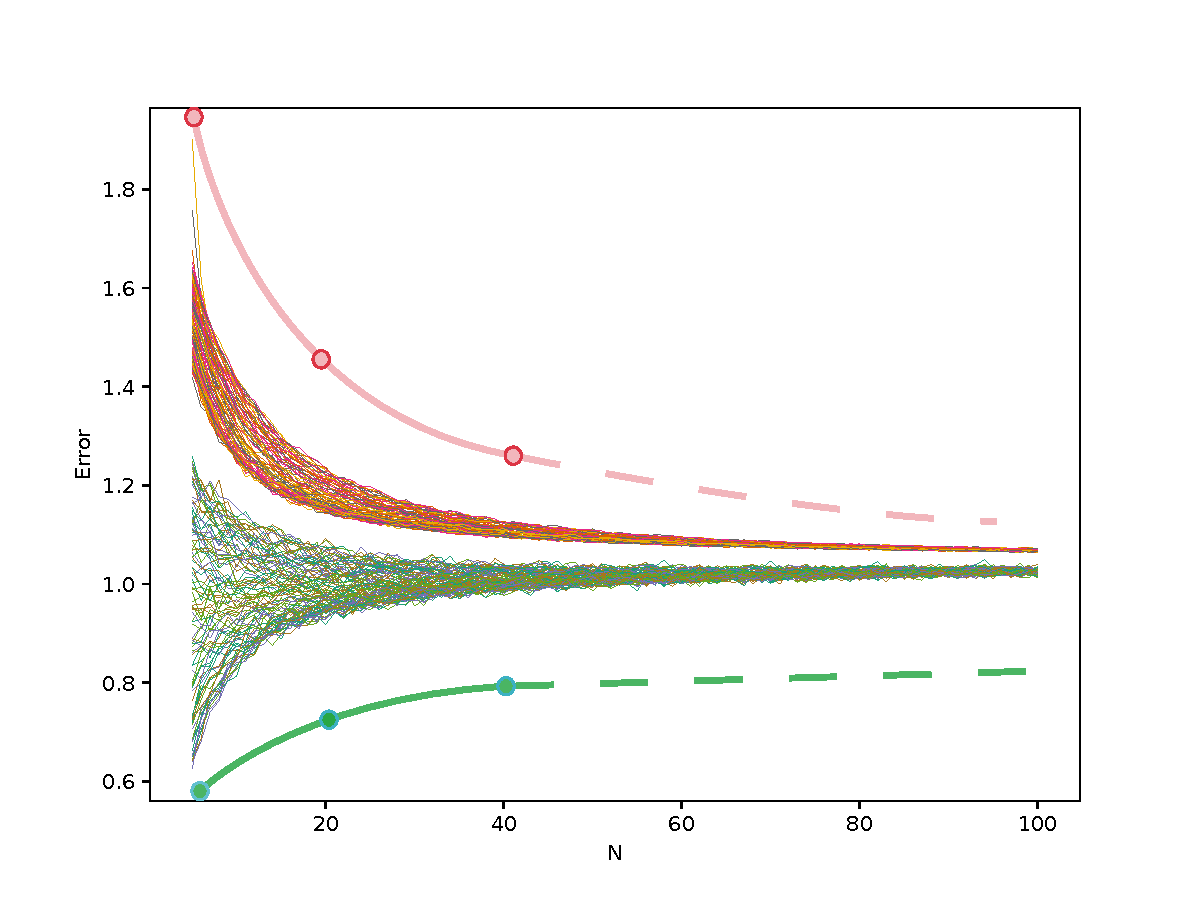
\includegraphics[width=\textwidth]{figures/lc.pdf}
  \end{minipage}
\end{frame}

\begin{frame}{Learning Curves Extrapolation}
  \begin{minipage}{0.5\textwidth}
    \begin{itemize}
      \item<1> Parametric curve fitting (\textit{e.g.} power law, exponential and logarithmic models)
      \item<2> Marco's presentation about parametric fitting being really tough!
      \item<3> Non-monotonic learning curves.
    \end{itemize}
  \end{minipage}%
  \begin{minipage}{0.5\textwidth}
    \centering
    \includegraphics<1-2>[width=\textwidth]{figures/lc.pdf}
    \includegraphics<3>[width=\textwidth]{figures/nonmonlc.png}\cite{looga}
  \end{minipage}
\end{frame}

\begin{frame}{Research Questions}
  \centering
  \color{Pink} \textit{Question 1.} \color{Black} What is the performance gain of a completely data-driven learning curve extrapolation compared to conventional parametric learning curve fitting? 

  \vspace{1cm} 

  \color{Pink} \textit{Question 2.} \color{Black} Performance of a data-driven learning curve for non-monotone curves?
\end{frame}

\section{Problem Definition}
\begin{frame}
	\centering
	\pr
\end{frame}

\begin{frame}{Learning Problem}
  \begin{minipage}{0.5\textwidth}
    \only<1>
    {
    For a learning task $T_i$
    \begin{itemize}
      \item $\risk = \lc(\nsamp) + \varepsilon$,
    \end{itemize}
    }
    \only<2>
    {
    With the objective as,
    \begin{itemize}
      \item $\hat{\model} = \min_{\model\in\hilbert} \loss(\model,\risk) + g(||\model||_\hilbert)$
    \end{itemize}
    }
    \only<3>
    {
    With the objective as,
    \begin{itemize}
      \item $\hat{\tilde{\model}} = \min_{\tilde{\model}\in\hilbert} \loss(\tilde{\model},\risk) + g(||\model||_\hilbert)$
    \end{itemize}
    }
    \only<2>
    {
    Kernel Ridge learner is obtained via \textit{Nonparametric Representer Theorem}\cite{scholkopf2002a}
    \begin{itemize} 
      \item $\model(\cdot)=\sum^{\samplr}_i\alpha_i k(\cdot,\sampi)$
    \end{itemize}
    }
    \only<3-4>
    {
     If you assume $\tilde{\model}= \model + h$ where $h\in span\{\psi_p\}$ and $\{\psi_p\}_{p=1}^\samplr$ via \textit{Semi-parametric Representer Theorem }\cite{scholkopf2002a}
     \begin{itemize}
       \item  $\tilde{\model}(\cdot)=\sum_i^\nsamplr\alpha_i k(\cdot,\nsampi)+\sum_j^\numlc\beta_j\psi_j(\cdot)$
     \end{itemize}
     }
    \includegraphics<5>[width=\textwidth]{figures/noise_1.pdf}
  \end{minipage}%
  \begin{minipage}{0.5\textwidth}
    \only<1-3>
    {
    \begin{itemize}
      \item<1> $\varepsilon\sim\mathcal{N}(0,\sigma^2)$ 
      \item<2> $\hilbert$ Reproducing Hilbert Space
      \item<2-3> $\model$ Model
      \item<2-3> $\tilde{\model}$ Model with additional functions
      \item<3> $\psi_p$ additional available functions
    \end{itemize}
    }
    \includegraphics<4>[width=\textwidth]{figures/lc.pdf}
    \includegraphics<5>[width=\textwidth]{figures/learningcurve2.pdf}
  \end{minipage}
\end{frame}

\section{Initial Questions}
\begin{frame}
	\centering
	\res
\end{frame}

\begin{frame}{Significance of $\boldsymbol{\alpha}$}
  \begin{minipage}{0.5\textwidth}
    \only<1>
    {
      %\includegraphics[width=\textwidth]{figures/eg.pdf}
    }
    \only<2-3>
    {
    \begin{itemize}
    \item $\model_1:=\sum_j^\numlc\beta_j\psi_j(\cdot)$
    \item $\model_2:=\sum_i^\nsamplr\alpha_i k(\cdot,\nsampi)+\sum_j^\numlc\beta_j\psi_j(\cdot)$
    \item $\model_3:=\sum_i^\nsamplr\alpha_i k(\cdot,\nsampi)$
    \end{itemize}
    }
  \end{minipage}%
  \begin{minipage}{0.5\textwidth}
    \only<2>
    {
    Statistical Hypothesis Testing
    \begin{itemize}
      \item t test
      \item f test
      \item chi square test
      \item Wilcovon Rank-Sum 
      \item $\vdots$
      \item \color{Pink} Cramer Von Misses
    \end{itemize}
    }
    \only<3>
    {
      Controlled Environment ($\sigma$, $\boldsymbol{psi}$ look at the Extrapolation+Interpolation Error populations.
      Informative $\boldsymbol{\psi}$ 
      \begin{itemize}
        \item All combinations are significantly different $\to$ $\sigma=0$
        \item $\model_1-\model_2$ not different, but other combinations are different  $\to$ $sigma\neq$
      \end{itemize}
    }
  \end{minipage}
  \only<4>
  {\color{Pink} Final verdict: Go with the more flexible method!}
\end{frame}

\begin{frame}{Selection of $\boldsymbol{\psi}$}
  \begin{minipage}{0.5\textwidth}
    \only<1-2>
    {
    \begin{itemize}
      \item<1> Using the raw curves
      \item<2> Extracting information from learning curves...
    \end{itemize}
    }
  \includegraphics<3>[width=\textwidth]{figures/sine.pdf}
  \end{minipage}%
  \begin{minipage}{0.5\textwidth}
    \begin{itemize}
      \item<3> Functional ($\mR^d\to\mR$) Analysis
      \item<3> equal spacing, same region etc...
    \end{itemize}
  \end{minipage}
  \only<4>
  {
  \color{Pink} Final verdict: functional PCA usage is especially important for noisy curves due to smoothing introduced!
  }
\end{frame}

\begin{frame}{How does it look now?}
  \begin{minipage}{0.5\textwidth}
    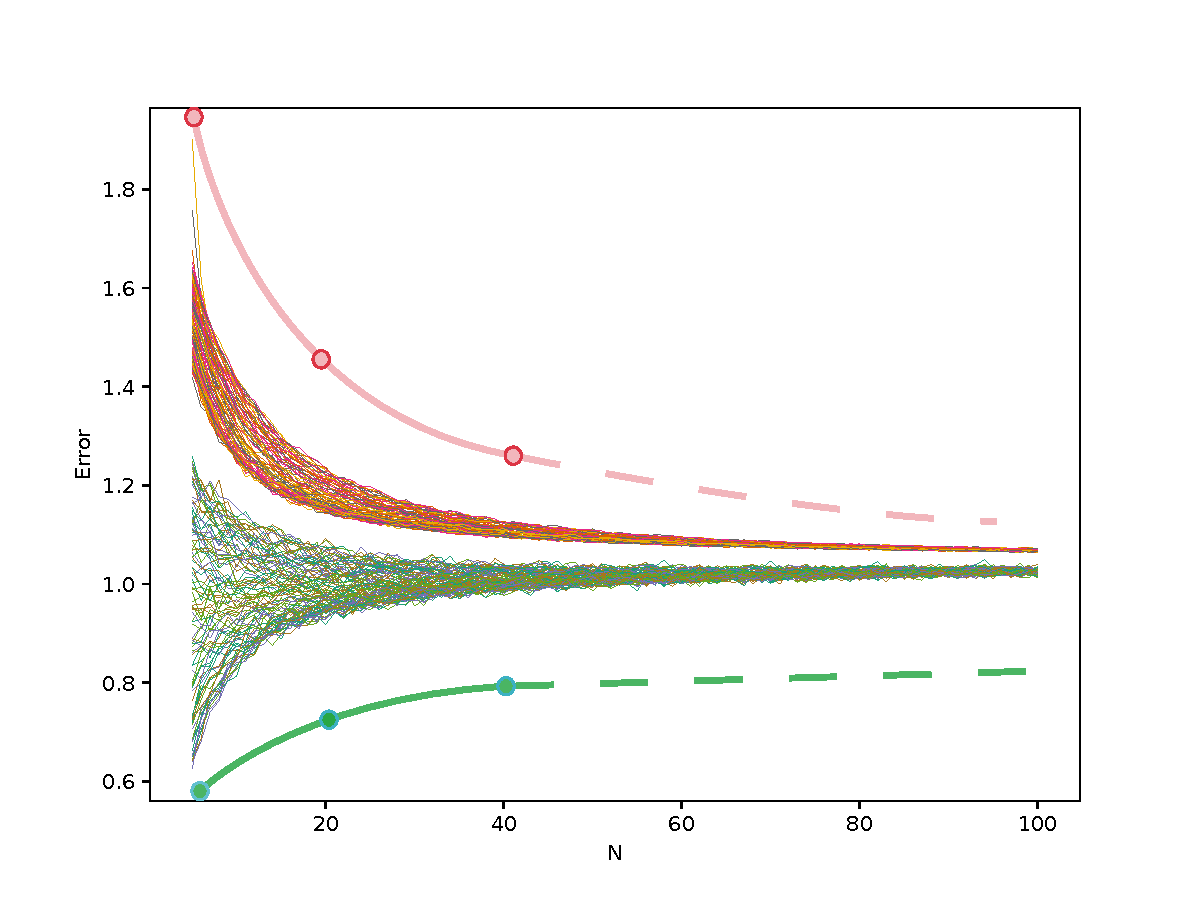
\includegraphics[width=\textwidth]{figures/lc.pdf}
  \end{minipage}%
  \begin{minipage}{0.5\textwidth}
    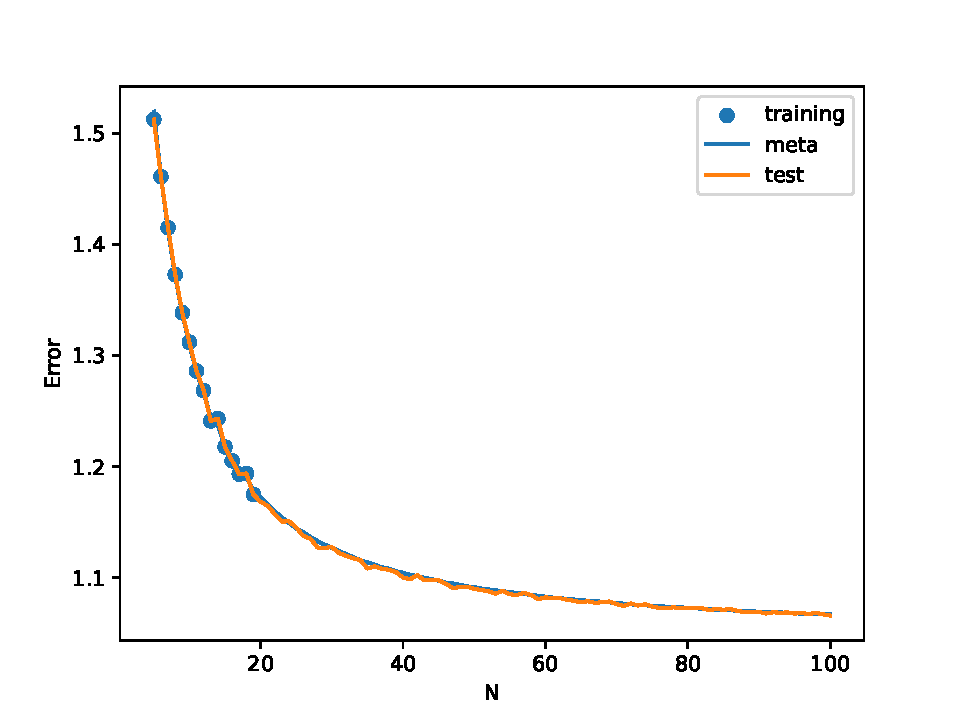
\includegraphics[width=\textwidth]{figures/lr_2_pca.pdf}
  \end{minipage}

\end{frame}

\begin{frame}{Curve Fitting Problems}
  \begin{minipage}{0.5\textwidth}
    \begin{itemize}
      \item<1> Marco's talk
      \item<1> $p(x,a,b,c):=a*e^{(b*x)}+c$
    \end{itemize}
  \end{minipage}%
  \begin{minipage}{0.5\textwidth}
    \begin{itemize}
      \item<2> De Facto $\to$ Levenberg–Marquardt method (Gradient Descent + Gauss Newton)
      \item<2> Playing with the internal optimizer parameters. (Not helping!)
    \end{itemize}
  \end{minipage}
  \only<3>{
\color{Pink} Final verdict: Try various optimizers and various runs get the best one!  
}
\end{frame}

\section{Plans}
\begin{frame}
	\centering
	\plans
\end{frame}

\begin{frame}{To Do}
	\centering
  \begin{minipage}{0.5\textwidth}
    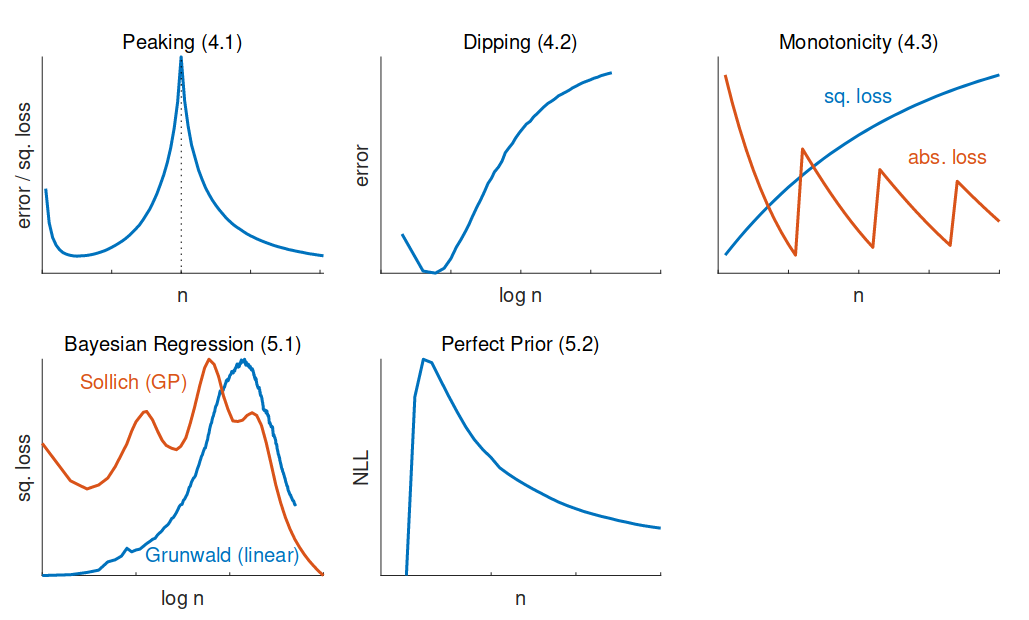
\includegraphics[width=\textwidth]{figures/nonmonlc.png}\cite{looga}
  \end{minipage}%
  \begin{minipage}{0.5\textwidth}
    \begin{itemize}
      \item Generating learning curve data
      \item Comparing performance of semi-parametric kernel ridge to parametric curve fitting in vari/us settings. (\textit{e.g.} changing hyper-parameters, $\prob_{X,Y}$, and learners...)
    \end{itemize}

  \end{minipage}
  \end{frame}


\begin{frame}
	\centering
  \thnx
\end{frame}

\end{document}
